\documentclass[a4paper, times, 12pt, ,onecolumn,oneside,top=1.0cm,bottom=1.0cm,left=1.0 cm,right=1cm]{article}
\usepackage{setspace} 
\usepackage{comment}
\usepackage{style}
\usepackage{multirow}
\usepackage{multicol}
\usepackage[ruled,vlined]{algorithm2e}
\usepackage{mwe}
\usepackage{wrapfig}
\begin{document}
%\pagestyle{plain} 
%\pagenumbering{arabic} 



\renewcommand\maketitle{
        \begin{center}
            \thispagestyle{plain}
            \noindent\rule{\textwidth}{3pt}\\
            \vspace*{0.2 in}
            \textbf{\LARGE  PhD Project Proposal for Qualification Exam : }\par
            \vspace*{0.5 in}
            \textbf{\large Eye-tracking Based Visual Attention Prediction with Computational Attention Model in Natural Viewing Environment and Its Application in Medical Screening}
           \vspace*{0.2 in}
            \noindent\rule{\textwidth}{1 pt}
            \textbf{\normalsize Po-Hsuan Huang}\\
            \vspace*{ 0.05 in}
            \textbf{\small Neuroscience Graduate Program, University of Southern California, USA}\\
            \vspace*{0.05 in}
            \texttt{\normalsize pohsuanh@usc.edu}\\
            \vspace*{0.1 in}
            \textbf{\normalsize Advisor :  Dr. Laurent Itti}

            
        \end{center}
    }
\maketitle
\tableofcontents


\section{Introduction}
\subsection{Background}
Eye-tracking technology provides a safe, fast and inexpensive gateway to the states visual attention of humans in natural environments. Vision-guided attention and oculomotor behaviours in various scenes and environments recruits neural circuits extensively and therefore provide valuable information about a person's mental states and mental well-beings. For example, scientists showed that combining eye-tracking technology and computational modeling of human visual circuitry can detect anomaly that are correlated to Attention Deficit Hyperactivity Disorder(ADHD)\cite{pmid22926163}, Fetal Alcohol Spectrum Disorders(FASD)\cite{fneur.2019.00080}, and Autism Spectrum Disorder (ASD)\cite{pmid26593094} when participants are positioned to watch videos without prerequisite goal to mimic task-free, natural viewing experience. Therefore, having a good computational model of vision guided attention in natural viewing environment is desirable not only because it help us better understand the working mechanism of visual attention allocation in dynamic visual environment, but also provide a generalizable method to help doctors diagnose neurological disorders.

However, previous methods suffers two major constraints to either become more accurate, or deal with elusive, emerging neurological disorders such as toxic stress. In our research specifically, we are going to use toxic stress data set to demonstrate the significance of our proposal. Accumulating studies over decades have provided evidence supporting that adverse childhood experiences (ACE) is highly associated with a multitude of physiological and mental developmental diseases. ACE can leave permanent, irreversible co-occurring damages to multiple body systems which lead to life-long negative impact on a multitude of health risk factor domains.\cite{ACE}\cite{ACE1}\cite{ACE2} Therefore, a valid and reliable evaluation tool of neurological disorders for infants that can profoundly change a person's life expectancy and life quality is highly sought after.

\subsection{Problems}
First of all, these models relies on accurate labels of the data. In real world medical screening, misdiagnosis of mental illness is not rare. In particular, medical data sets usually recruit limited number of participants, which magnifies the model bias caused by mislabeling. These labels that contains incorrect labels are called 'weak' labels. Developing a semi-supervised algorithm that utilize inherit consistency of embedded representation will provide robustness in our predictions to avoid over-fitting to out-liers and incorrect labels. The second fold of the benefit of using semi-supervised learning techniques on medial data is that is that it provides a way to recruit 'soft' labels to the training data set. Soft labels are crucial to eye-tracking data sets because eye-tracking data are inexpensive to collect, while diagnosis from experts are expensive. The second constraint is that these computational models relies on artificially defined salinecy features for pixel level visual information processing, and semantic features for mid to high level cognitive visual information processing based on the best knowledge of human experts. These hand-crafted features, although interpretable, might failed to capture important features that is outside experts' knowledge and expectations.
As a result, it poses constrains on maximizing classification accuracy and  minimizing risk of mis-classification. Alternatively, we can train the features with massive amount of data to optimize the accuracy of classification of potential patients of neurological disorders. However, it is usually expensive to get massive amount of medical data. 

\subsection{Proposed Solutions}
My proposal aims to solve two major problems to develop more accurate eye-tracking based screening tools: First, I would like to use RANSAC inspired semi-supervised learning method to overcome lack of labeled data and issue of weak labels. Second, I would like to develop a computational model based on state-of-the-art deep neural networks to predict visual attention of patients in videos.

\subsection{Significance}
I expect my research to make significant contribution to computer aided diagnosis. A better computational model of visual attention will help doctors make more accurate diagnosis of neurological or attention-related disorders at early stage. In particular, we are collaborating with doctors in Children Hospital of Los Angeles to try to diagnose toxic stress caused by adverse childhood experience.    

\section{Aim 1 : RANSAC inspired classification algorithm for accurate prediction of weakly labeled medical data} 
    
\subsection{Introduction}
Random Sampling Consensus (RANSAC)\cite{10.1145/358669.358692}  is a empirical method to exclude samples that does not fit the model's assumptions, such that the fitting is not compromised by outliers. To illustrate the idea, we will use linear regression as an example. The algorithm can be described as followed :

\begin{algorithm}
\SetAlgoLined
 1: Randomly select the minimum number of points required to determine the model parameters.
 
 2: Solve for the parameters of the model.
 
 3: Determine how many points from the set of all points fit with a predefined tolerance $\epsilon$.
 
 4: If the fraction of the number of inliers over the total number points in the set exceeds a predefined threshold $\tau$, re-estimate the model parameters using all the identified inliers and terminate.
 
 5: Otherwise, repeat steps 1 through 4 (maximum of \textit{N} times).
\caption{\textbf{ Linear Regression with Random Sampling Consensus (RANSAC)  }}
 \end{algorithm}
    
It was first used in fitting problems that only requires few correct samples to determine parameters of a model, hence percentage of outliers is not limited. Most shallow classifiers are sensitive to anomaly and usually requires manual data cleansing to remove outliers. However, manually inspect and cleanse training data can be difficult and costly even for small data set because labeling samples can be hard for rare medical diseases. As shown in figure 5, the linear regression cost function is sensitive to outliers in the training set(orange color), which leads to aberrant fitting line that is far from the ground truth underlying pattern if blue dots are also included in the training set. By selecting the samples in the training set randomly, we get the chance to have a clean subset free of outliers that ultimately help us to find the correct fit with minimum possible standard deviation. The algorithm is shown to have a guaranteed probability of conversion within N iterations.    
Figure 1 shows how RANSAC helps find a robust fitting parameters by detecting out-liers. Here the goal is to fit a straight line that best describe the data. We can see from this example that the two out-liers on the left side and right side of the line consists of all the other dots are going to undermine the fitness of line, and therefore it is favorable to exclude them from the training set. Here we explain how RANSAC achieves that. First, 2 samples are selected randomly (orange dots in red circles). Second, the parameters of the line $\tho_{0}$ and $\sigma_{0}$ are solved from the two points. Then, out-liers and in-liers are determined by a confidence interval d from the center of line. The orange dots are in-liners, and the blue dots are out-liers. Finally, if the number of in-liers exceeds a threshold value, then we reiterate the procedure again with all in-liers. Otherwise, re-samples 2 points and start again. Repeat the procedure until the accuracy surpass a termination criterion. As you can see from the illustration, the fitting line of the 7 orange dots will be more aligned with the ground truth distribution than the line determined by the two dots in red circles. RANSAC is guaranteed to converge given sufficient trials.
\begin{wrapfigure}{r}{0.45\textwidth}
\begin{center}
  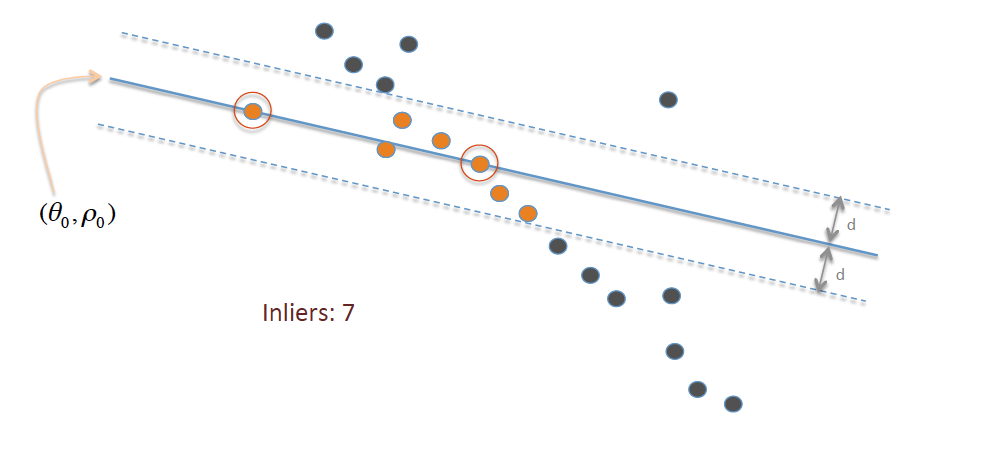
\includegraphics[scale=0.25]{imgs/intro_2.png}
  \caption{\textbf{Illustration of Random Sampling Consensus:  Robust Fitting }}
\end{center}
\end{wrapfigure}

  \subsection{Rationale/Premise}
    In this paper, we proposed to apply RANSAC as a classification algorithm to exclude incorrect labels(Random Sampling Phase) and find manifold.(figure 2) Using RANSAC with SVM has been applied to detect annotation errors for robust fitting and detect hard examples in optical object recognition \cite{BMVC2015_168}. Nishida and Kurita \cite{4761280} used RASNAC with SVM to find the most generalizable subset of samples to solve the problem of learning with large number of examples. In this paper, we try to use RANSAC to solve two problems at once. 

Our ACE data set is challenging because many important knowledge are unknown to the pediatricians : The lack of medical tracking records of children patient prevent us from getting accurate class labels but inexact risk label defined by composite scores empirically. The lack of pathological understanding prevent us from designing optimal features for machine learning. The chronic nature of the disorder make it difficult to observe dissimilarity between healthy participants and affected participants at the early stage of the disorder. 

To justify our algorithm we first examine the hypothesis on four synthetic data set under various mislabelling and manifold entangling scenario. Secondly, we tested our algorithms on popular medical data sets whose samples contains unknown percentage of outliers. We compare the f1 score of our algorithm with state of the art SSL-SVM models.

Additionally, we further reinforce the confidence of our model by predicting other attributes such as sex and age of the participants of ACE data set. Finally,  We believe the accuracy of our model will increase significantly as the increase of data size and label accuracy thanks to more track records of children becomes available. 

As shown in Fig. 2, the pipeline consists of three major steps. \textbf{(a)Feature extraction} The video clippets are processed to extracts oculomotor features (Saccade Peak Velocity, Saccade, Velocity, Saccade Acceleration, Fixation Duration, Pupil size), saliency features (Color,Flicker,Intensity,Motion,Orientation), semantic features(objectness, background-ness, animated objects, human face), and similarity to controlled distribution at each attention time stamp which is defined as end of saccade. In total, there are 15 channels and say $\tau$ attention time stamps. The size of the data is now $15  \times \mathcal{T}$.   \textbf{(b)Dimentionality reduction} The 2 dimensional features are then summarized with histogram to reduce the size $\mathcal{T}$ to a fixed value. After rescaling and extremua removal, the summarized histogram reduced the temporal dimension and only represents the distribution of responsiveness to each feature. We assign 9 bins for each channel and the total size of the feature becomes 15 $\times$ 9 \textbf{(c) RANSAC Classification} We deploy different RANSAC algorithm to remove outliers from the final training set. The base classifiers predicts confidence value of each labels. If the confidence of a prediction is high for a sample, we include sample and predicted label into the training set of the next iteration. The RANSAC process is repeated after validation until results that meets the \textbf{ (d) convergence criteria}.
\begin{wrapfigure}{0.45\textwidth}  
\centering
     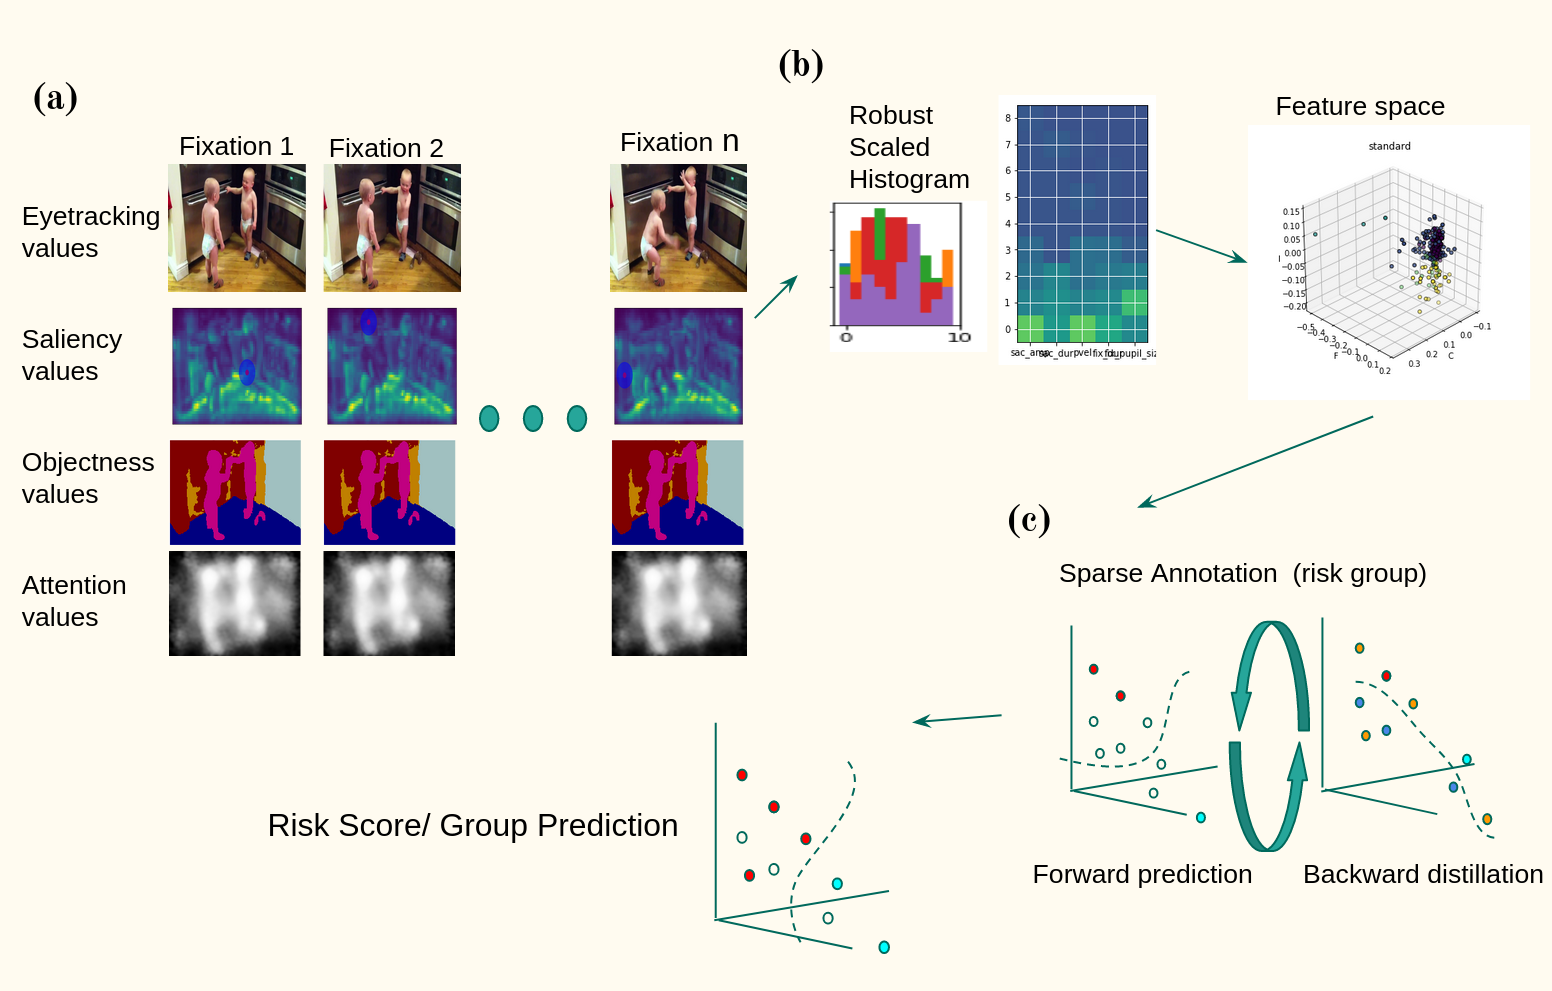
\includegraphics[scale = 0.25]{imgs/our_pipeline.png}
  \caption{\textbf{An overview of the pipeline of our proposed model for toxic stress risk prediction} }
\end{wrapfigure}
\clearpage
    

\subsection{Objective}
Our algorithm mimics the original RANSAC fitting algorithm that continuously recruit inliers inside the predefined error tolerance $\epsilon$ to find the underlying data manifold. In the meantime, stochastic natural of random sampling techniques can help avoid learning from incorrect labels. Incorrect labels can significantly disrupt SSL algorithm and many outlier sensitive classifiers such as SVM or KNN. 

We propose two different varieties of RANSAC classification algorithms. The first algorithm is inspired by semi-supervised learning algorithm from object recognition task of computer vision. It is a general rule that pseudo labels generated by algorithms can fine-tune the model itself because increased amount of training data provides additional information. Accuracies of these models improve incrementally over iterations of pseudo labeling as training data accumulate. 
 In Fig. 3, the algorithm 1 for RANSAC algorithm consists of iterations of three-step serial process of supervised training, validation, and generalization. \textbf{Supervised learning step :} A fraction of the weakly labeled data is sampled as the training samples, and the rest of the labeled data becomes the validation set. If the training from the sample set generates acceptable accuracy score, the trained classifier is used predict confidence values of the validation set. Otherwise, we re-sample training set from the labeled data set \textbf{Validate Generalization:} The fitted model is then used to predict confidence values of the validation set. The in-liers of the validation set are temporarily added to the training set and refit the model. The inclusion becomes permanent if the accuracy score improves. Otherwise, restart the whole process from step 1. \textbf{Generalization step:} Finally. the fitted model is used to predict the unlabeled data set. Since our model has already removed out-liers, and confidence measure calibrated. It's prediction of unlabeled data is supposed to be more accurate than plain supervised training. We further refine the model parameters by giving confidence scores to the unlabeled data points, and repeat the in-lier detection-refit step to incrementally improves the predictive power of the model. Finally. the whole unlabeled data set is classified using \textit{argmax} on the confidence score. The whole three-step process is run $\mathcal{N}$ times and the model of the best accuracy is kept as the final model. As N increase the model is bound to converge.   
\begin{figure*}
  \centering
  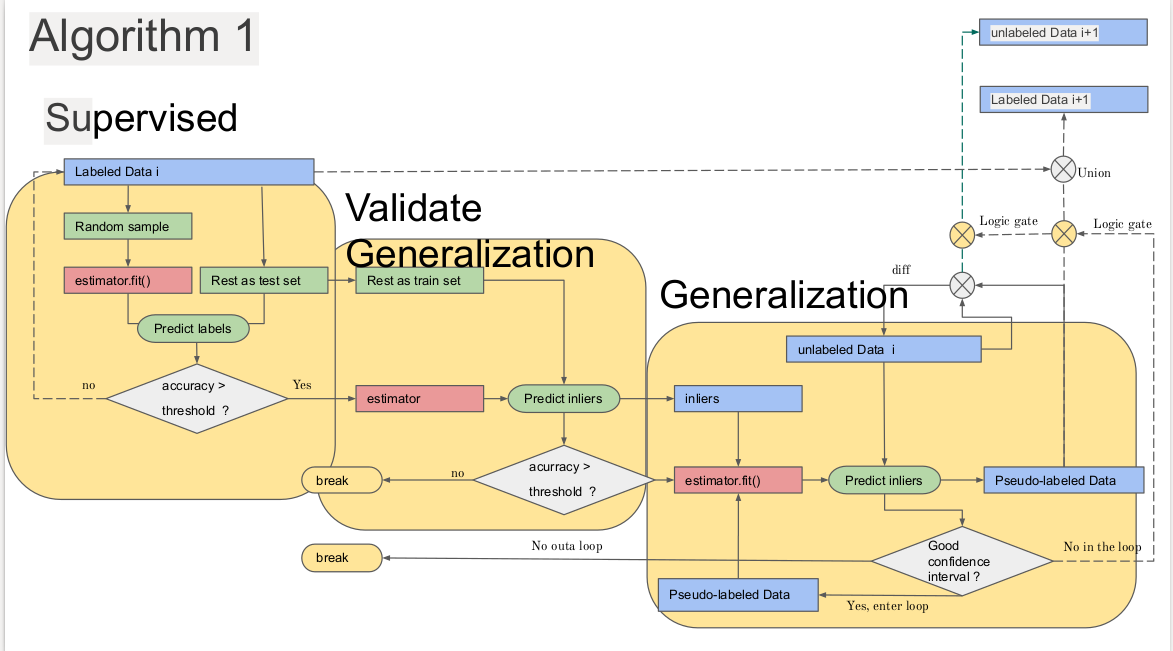
\includegraphics[scale = 0.35]{imgs/RSVM1_diagram.png}
  \caption{\textbf{Flow Chart of RANSAC Classification Algorithm 1}
 }
\end{figure*}

The second RANSAC algorithm we proposed are conceptually simple.(Fig. 4) It is similar to \textit{Boostrap Aggregation (Bagging)}. First, an ensemble of base learners are instantiated by training them with randomly sampled subsets. The sampling can be irreplaceable to increase learner diversity. The base learners ensemble then make prediction about unlabeled data.Predefined consensus mechanism estimates confidence score along with labels. The predictions of the ensemble then go through 'consensus forming' to assign labels to unlabeled data.  In our implementation, unanimous consensus, where all base learners' prediction agree is used to recruit samples. Iterative selecting the most confident unlabeled samples reduced the negative effect of out-liers.   


 The algorithm 2 (Fig. 4) is similar to Bootstrap Aggregation Algorithm(Bagging) but with subtle difference in its consensus step. Initially there is a small labeled data set marked in dark blue, and a large unlabeled data set marked in light blue. $\mathcal{N}$ base classifiers are fit with randomly sampled data from the labeled set with a fixed sampling rate. The $\mathcal{N}$ classifiers are then  predict the class of all unlabeled data in parallel through various consensus algorithm such as absolute majority, max probability, or unanimous consensus just like Bagging. However, in this algorithm we add the most confident samples alone with the predicted labels (pseudo labels, soft labels) to the labeled data set in the second iteration. We repeat the process until no more high confidence labels can be found. The accuracy of the method should do better than begging since the soft labels increase the size of training set. To predict the unlabeled data points, we use \textit{argmax} on the unlabeled data set.
 \begin{figure}{H}
   \centering
  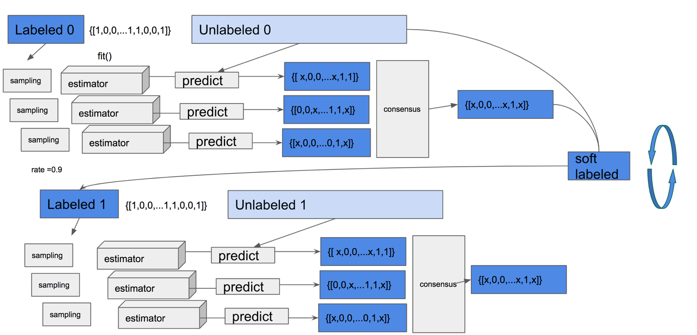
\includegraphics[scale = 0.5]{imgs/algo2.png}
  \caption{ \textbf{Flow Chart of RANSAC Classification Algorithm 2}}
    \end{figure}

\subsection{Experiment Designs}

\subsubsection{Experiment 1 : Synthesized Data sets}
Medical data labels suffer from two type of challenges : inaccuracy and incompleteness. Label inaccuracy is common for medical data set due to mislabeling. Incompleteness usually comes from difficulty to collect data from confirmed cases of rare diseases that interest us. We evaluate the average accuracy of binary classification of our two RANSAC algorithms under various ratio of incorrect labeling and labeled data/unlabeled data. The difficulty of SSL can be described by two factors: mislabelling ratio and test-split ratio. Difficulty of classification increase as mislabelling rate and test-split rate increase. The two factor spans a 2D space that describes large amount of weak labeling scenario that realistic data sets might belong to. We conducted extensive grid search of the whole label-quality space by computing mean of average score of RANSAC models of 10 trails. The evaluation is conducted on three synthesized 2D data set of various manifold structure. Moon shape data set is a case where two classes are separable and the manifold structure is non-trivial. Circle data set consists of two concentric circles, where a bigger circle is surrounding the smaller circle. In this case the manifold is more complex. Finally the overlapping data set consist of two partially overlapping blobs of random shapes. There isn't a manifold can separate the two classes. The qualitative experiment will allow us to define the working domain where models perform the best. Accuracy measurement cross parameter domain will help us define the best working area of the algorithms. We tested SVM and Multi-layer Perception(MLP) as base learner for both RANSAC algorithms to ensure the our algorithm are applicable to different base classifiers.

We also visualized the training iterations of RANSAC 1 and RANSAC2 algorithms to examine and verify if the learning mechanisms work as we hypothesized. 

\subsubsection{Experiment  : UCI Medical Data sets}
Three Medical data sets from UCI machine learning repository are used in the experiment.  These data set shares same difficulties we faced with Toxic stress data set. The challenges are class imbalance, limited data size, and ambiguous data manifold. However, we can actually evaluate the performance of our algorithms since these data set provides ground truths. In addition, these data sets are widely used as benchmarks by machine learning algorithms. We compared our result with other state-of-the-art models. We compare our RANSAC1-SVM , RANSAC2-SVM, and RANSAC2-MLP model to Transductive SVM and LapSVM. 

\subsubsection{Experiment 3 : Toxic Stress Data sets}
Eye-tracking, free-viewing paradigm has been applied to predict diseases such as ADHD, PD and FASD. Although we don't have perfect ground truths of toxic stress participants, we tested if RANSAC algorithms can improve prediction accuracy of sex and age of infants compared to the base learner without using RANSAC. The improvement of age prediction may suggest possible improvement of toxic stress risks prediction since toxic stress is associated with delayed cognitive maturation. On the other hand, improvement on sex prediction may suggests RANSAC's ability to find high confidence labels since sexual dimorphism in visual attention and oculomotor control should be minuscule before 1 year old.      
    
\subsection{ Preliminary Results}
\subsubsection{Experiment 1.1: Scenario Analysis for Synthesized Data sets}

In Figure 5, we analysis the accuracy of RANSAC algorithm 2 on the whole domain of label quality defined by Test-split ratio and mislabeling ratio. The higher the test-split ratio that more sparse the labeled data, therefore more generalization power will be needed. The higher the mislabeling the worse the fitting will be, so some outlier detection mechanism will be necessary. The upper row we inspect the performance of the proposed RANSAC algorithm 2 in easier label quality domain. The lower row we inspect the performance of the proposed RANSAC algorithm 2 in more difficult label quality domain. \textbf{center panel: } 3 layer Artificial neural networks model, of size 2-10-10-2 is used for evaluation. Three synthesized data distribution is tested for binary classification. The moon shape distribution and the two circle distribution has distinct decision boundary while the overlapped distribution doesn't have distinct decision boundary. The blue color means high accuracy, and the red color means low accuracy. The three columns from left to right shows the results of supervised training with clean labels, supervised method trained with noisy, sparse labels, and semi-supervised method trained with noisy, sparse labels. The results suggests the semi-supervised RANSAC algorithm 2 does improves the performance in both easy and difficult label quality domain. \textbf{right panel: } Constrained Support vector machine classifiers are trained in three different scenario. The three columns from left to right shows the results of supervised training with clean labels, supervised method trained with noisy, sparse labels, and semi-supervised method trained with noisy, sparse labels. The results show there is no distinct difference between supervised training and semi-supervised training in easier case. But the results slightly improved in the more difficult case. 
\begin{figure*}[ht]
\centering
  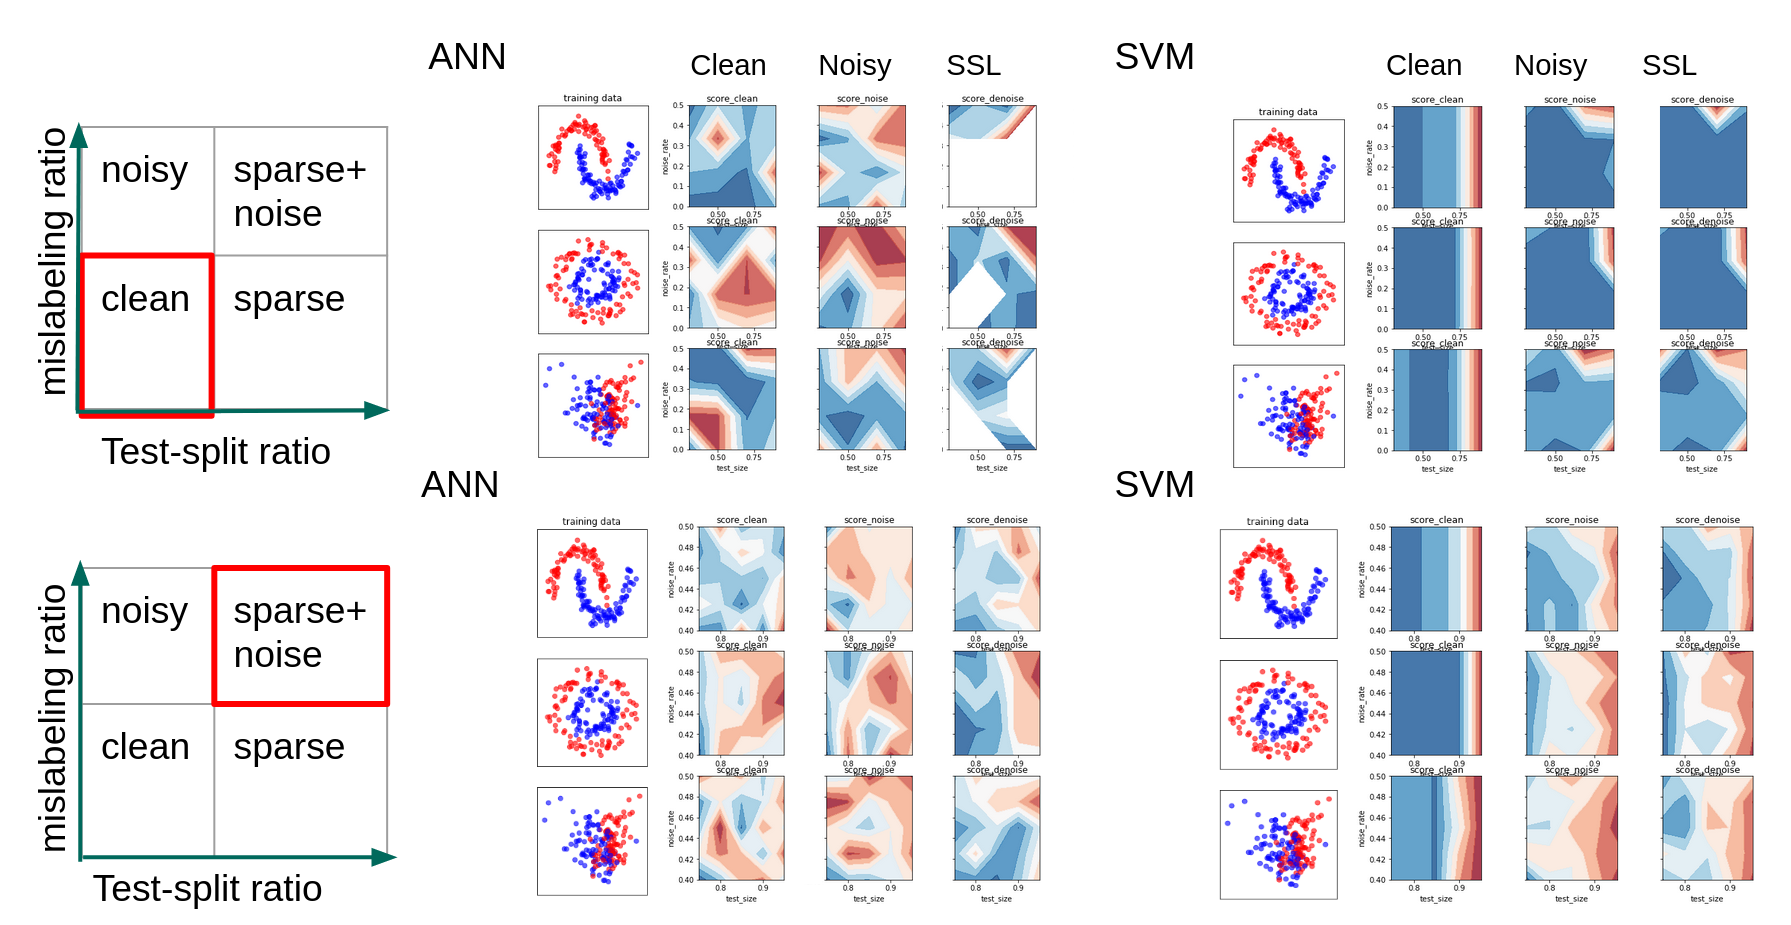
\includegraphics[scale = 0.2]{imgs/exp1_2-new.png}
  \caption{ \textbf{Label domain analysis} }
\end{figure*}

\subsubsection{Experiment 1.2: Visualize decision boundaries over iterations}
In Figure 6, we use Moon shape data set to visualize training iteration. Each row shows one iteration. We compare SVM trained with 10 \% ground truths, RANSAC algorithm1, RANSAC algorithm2,  RANSAC algorithm 3,  and SVM trained with 100 \% ground truths (columns from left to right ). The background color of each small subplot shows confidence estimate predicted by the models. It shows RANSAC algorithm 1 forms stronger and more accurate decision boundary for three evaluated base classifiers SVM, KNN, and MLP compare to RANSAC algorithm 2 and RANSAC algorithm 3. Algorithm 3 is similar to algorithm 2 but a backward outlier removal process is incorporated. The confidence estimate is consistant with our hypothesis that model forms better decision boundary if we select subset of samples that doesn't contain mislabelling outliers for training.      
\begin{figure}[ht]
  \centering
  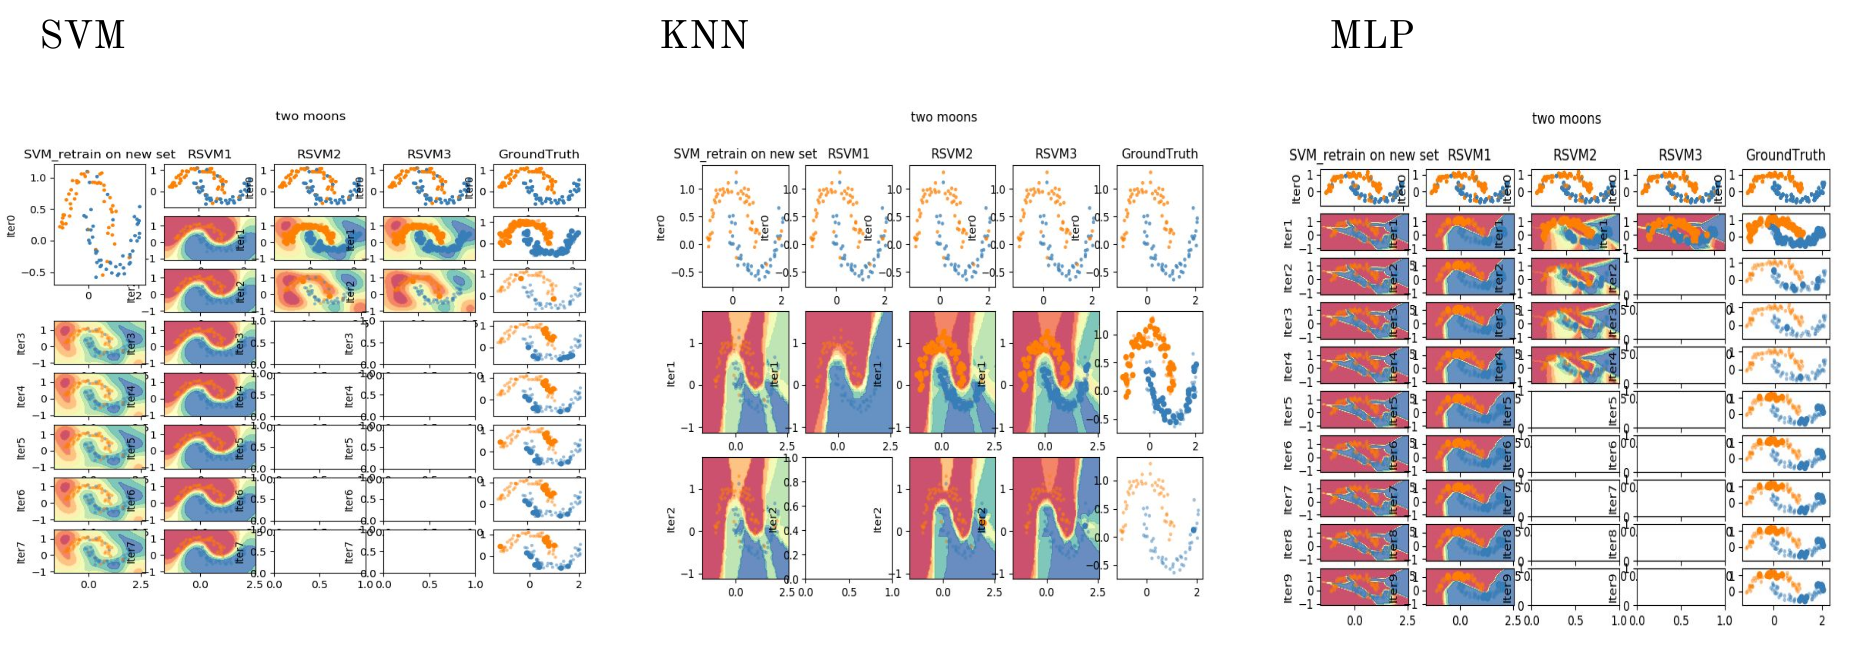
\includegraphics[scale = 0.25]{imgs/exp1-3-0.png}
  \caption{ \textbf{Iteration steps of RANSAC algorithms.}}
\end{figure}
\subsubsection{Experiment 3: Toxic Stress Data Sets}
Infants grow up at varying speed and delayed maturation is not unusual. Our experimental results on age prediction suggest RANSAC algorithm 1 helps predict age better than algorithm 2 and algorithm 3.(Figure 16) In fact, it predicts even better than SVM trained with 100 \% of labeled data. This suggests RANSAC improves prediction accuracy not only by reducing mislabeling, but it reduce weighting on low confidence, ambiguous samples.(Figure 7)

Finally, we use our model to predict and validate on toxic stress labels. The results are shown in figure 17. The yellow curve shows the prediction accuracy of RANSAC1-SVM when combining data across ages. Combining data across ages helps predicting toxic stress of 2 month old infants better when saliency features are used. It suggests free-viewing pattern of ACE victims differs from that of normal, healthy control groups in a consistent way throughout the critical developmental period. Since labels of infants of 2 months old are usually most inaccurate, finding consistent abnormal free-viewing behavioral pattern in saliency space in late infancy to childhood might help us predict ACE in early infancy. (Figure 8)       

\begin{figure}[H]
   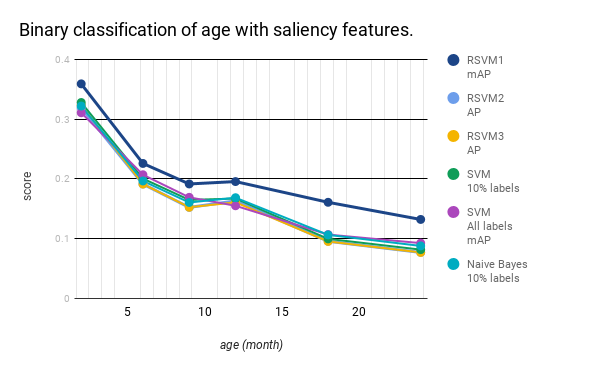
\includegraphics[width=0.53\textwidth]{imgs/exp3-2-1.png}
   \hfill
   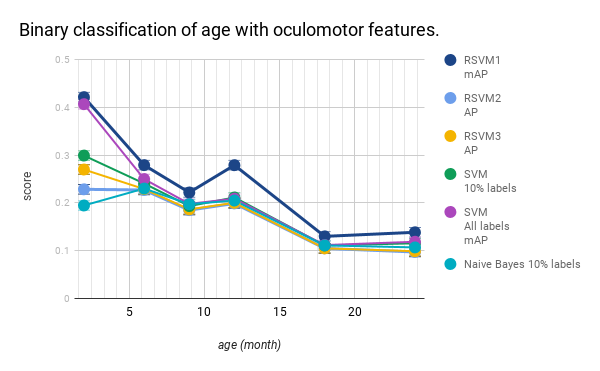
\includegraphics[width=0.53\textwidth]{imgs/exp3-2-2.png}
   \caption{ \textbf{Results of experiment 3.2 : Average precision of prediction of age} }
\end{figure}


\begin{figure}[H]
  \centering
  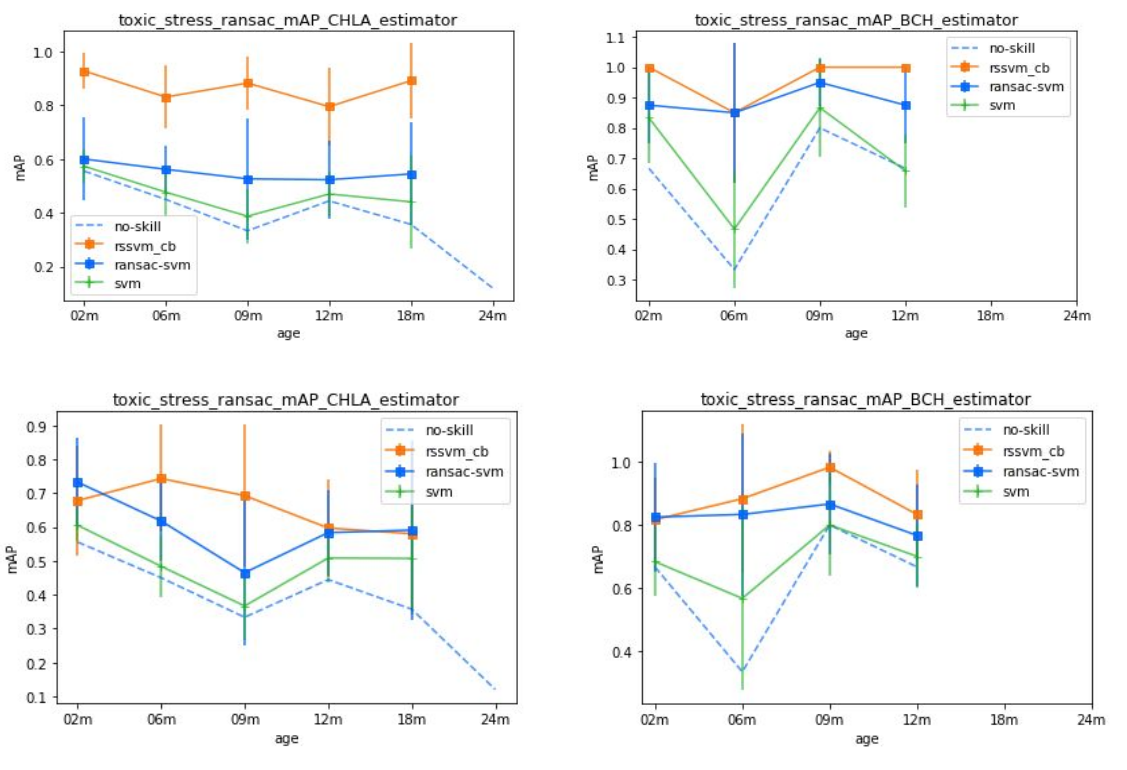
\includegraphics[scale = 0.4]{imgs/exp3-3.png}
  \caption{ The figure shows the results of experiment 3.3. Average precision of toxic stress classification with saliency features (panels in the top row) and oculomotor features( panels in the bottom row).}
    \label{fig:baseline}
\end{figure}

\clearpage
\section{Aim 2 : Deep Neural Network Modeling of Visual Attention in Videos }

\subsection{Rationale/Premise}
Advancement of deep neural networks in recent years has significantly improves the accuracy of gaze estimation and prediction in static scenes\cite{dg1}\cite{dg2}, as well as in dynamic  scenes.\cite{DGAZE} \cite{VSP-STRAN} \cite{Zhang_2017_CVPR}. Gaze estimation of static scenes usually leverages the features learned from object recognition data set, which contains massive amount of labeled images. Then, the model is fine-tuned with eye-gaze data set.
\begin{figure}{\textwidth}
  \centering
  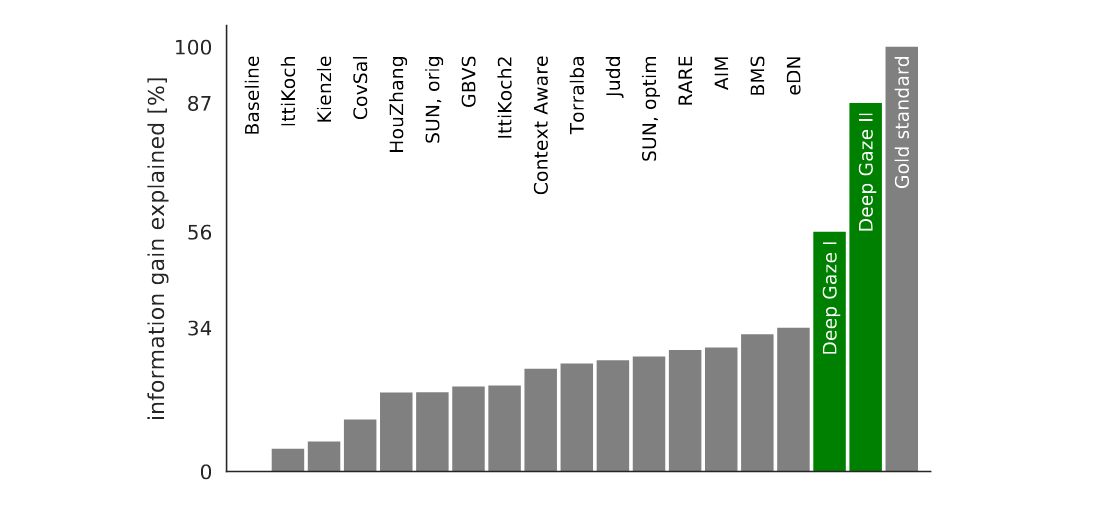
\includegraphics[scale = 0.4]{imgs/dg2_benchmark2.png}
  \caption{ The figure shows information gain explained as a  percentage of the gold standard model’s information gain relative to the baseline mode \cite{dg2}}
\end{figure}

On the other hand, although motions in dynamic scenes provides additional cues for gaze estimation, gaze estimation in dynamic scenes is still more challenging because of inconsistent movements around different foreground patterns, camera motions, and consideration of historical gaze scan paths. Extracting useful spatial-temporal features for gaze estimation in dynamic scenes is not only data intensive, but requires more understanding of how temporal patterns of multiple scales interact with spatial patterns. Recent development of generative adversarial networks has shown to be able to generate realistic data, and attention networks also bring advancement in video captioning, language translation, and motion recognition. Besides, recent advancement in representation learning and few-shot learning also provides numerous approaches to recognize and differentiate objects from very few labels. Our objective is to combine all these advantages provided by deep neural networks to overcome the aforementioned difficulties, and use our deep-learning based attention model develop better screening tool of attention related disorders. 

\subsection{Objective}

\subsubsection{Feature augmentation} Wang et. al. \cite{pmid26593094} showed that saliency features at object level and semantic level and help us understand behaviors of ASD and predict ASD patients better. (Fig.9). Likewise, we believe ACE can also lead to change in attention to object and semantic level saliency. We are going to incorporate object level and semantic level saliency feature in our present feature extraction pipeline alone with group similarity with young healthy adults in our future work. In 3 month we are going to implement and validate the efficacy of those semantic features, and then classify the unlabeled data with pseudo-labels.


\begin{figure*}[ht]
  \centering
  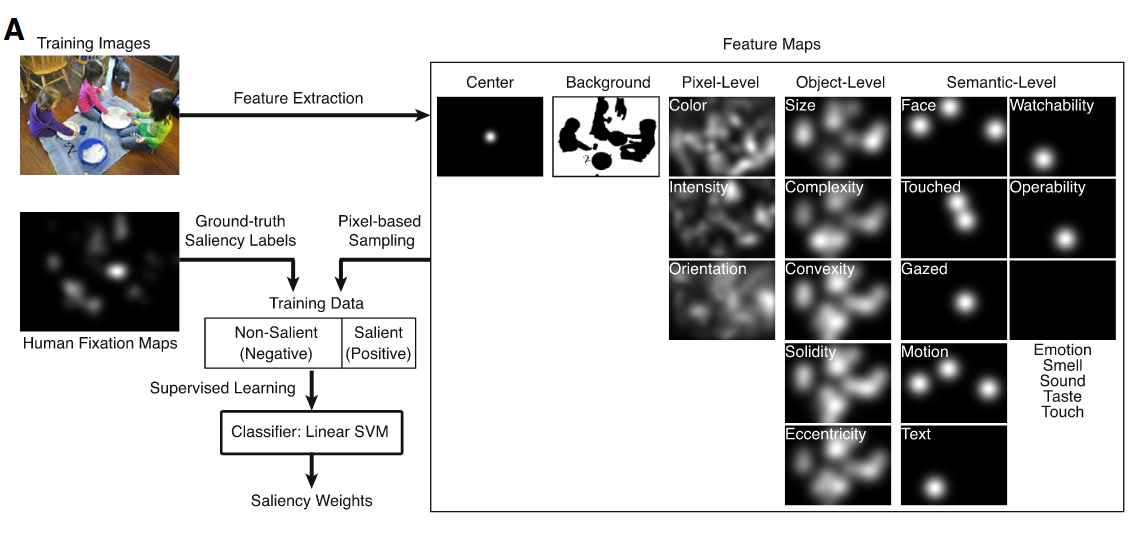
\includegraphics[scale = 0.4]{imgs/wang_pipeline.png}
  \caption{\textbf{Computational Saliency Model (Wang et. al. 2015)\cite{pmid26593094}}  An overview of the computational saliency model. We applied a linear SVM classifier to evaluate the contribution of five general factors in gaze allocation: the image center, the grouped pixel-level, object-level and semantic-level features, and the background. Feature maps were extracted from the input images and included the three levels of features (pixel-, object-, and semantic-level) together with the image center and the background. We applied a pixel-based random sampling to collect the training data and trained on the ground-truth actual fixation data. The SVM classifier output were the saliency weights, which represented the relative importance of each feature in predicting gaze allocation.}
  
  \end{figure*}

\subsubsection{Data augmentation} With the pseudo labels collected after \textbf{Feature augmentation}, we are able to have a small labeled data set with some wrong labels. In recent years, rapid development of deep-learning has shown tremendous success in representation learning. In particular, the generator-discriminator structure of adversarial learning make it possible to generate realistic data. With a massive amount of generated data, we should be able to improve the prediction accuracy of toxic stress risk substantially to the level of making our model a practical screening tool. 

\subsubsection{Data augmentation : Training the Spatial Temporal Attention model}
Recent breakthrough in attention mechanism, especially spacial-temporal attention neural networks(STA-NN), could help extract temporal saliency features and temporal oculomotor features that hasn't been discovered. For example, our current saliency map can predict probability of the location of foveation, but it cannot predict the viewing order. The other possible benefit is to determine the attentiveness of the human subject during fixation since fixation can be caused either by attention or idleness. With attention mechanism we should be able to give weightings to each time stamp during the fixation, and therefore we can analyze why some frames are more critical than the others. 

\subsubsection{ Prototypical coding : Triplet Loss}
Finally, utilize triplet loss function to achieve representation disentanglement in code space to facilitate convergence and reduce the required amount of data needed to train the model.



\begin{figure}[ht]
  \centering
  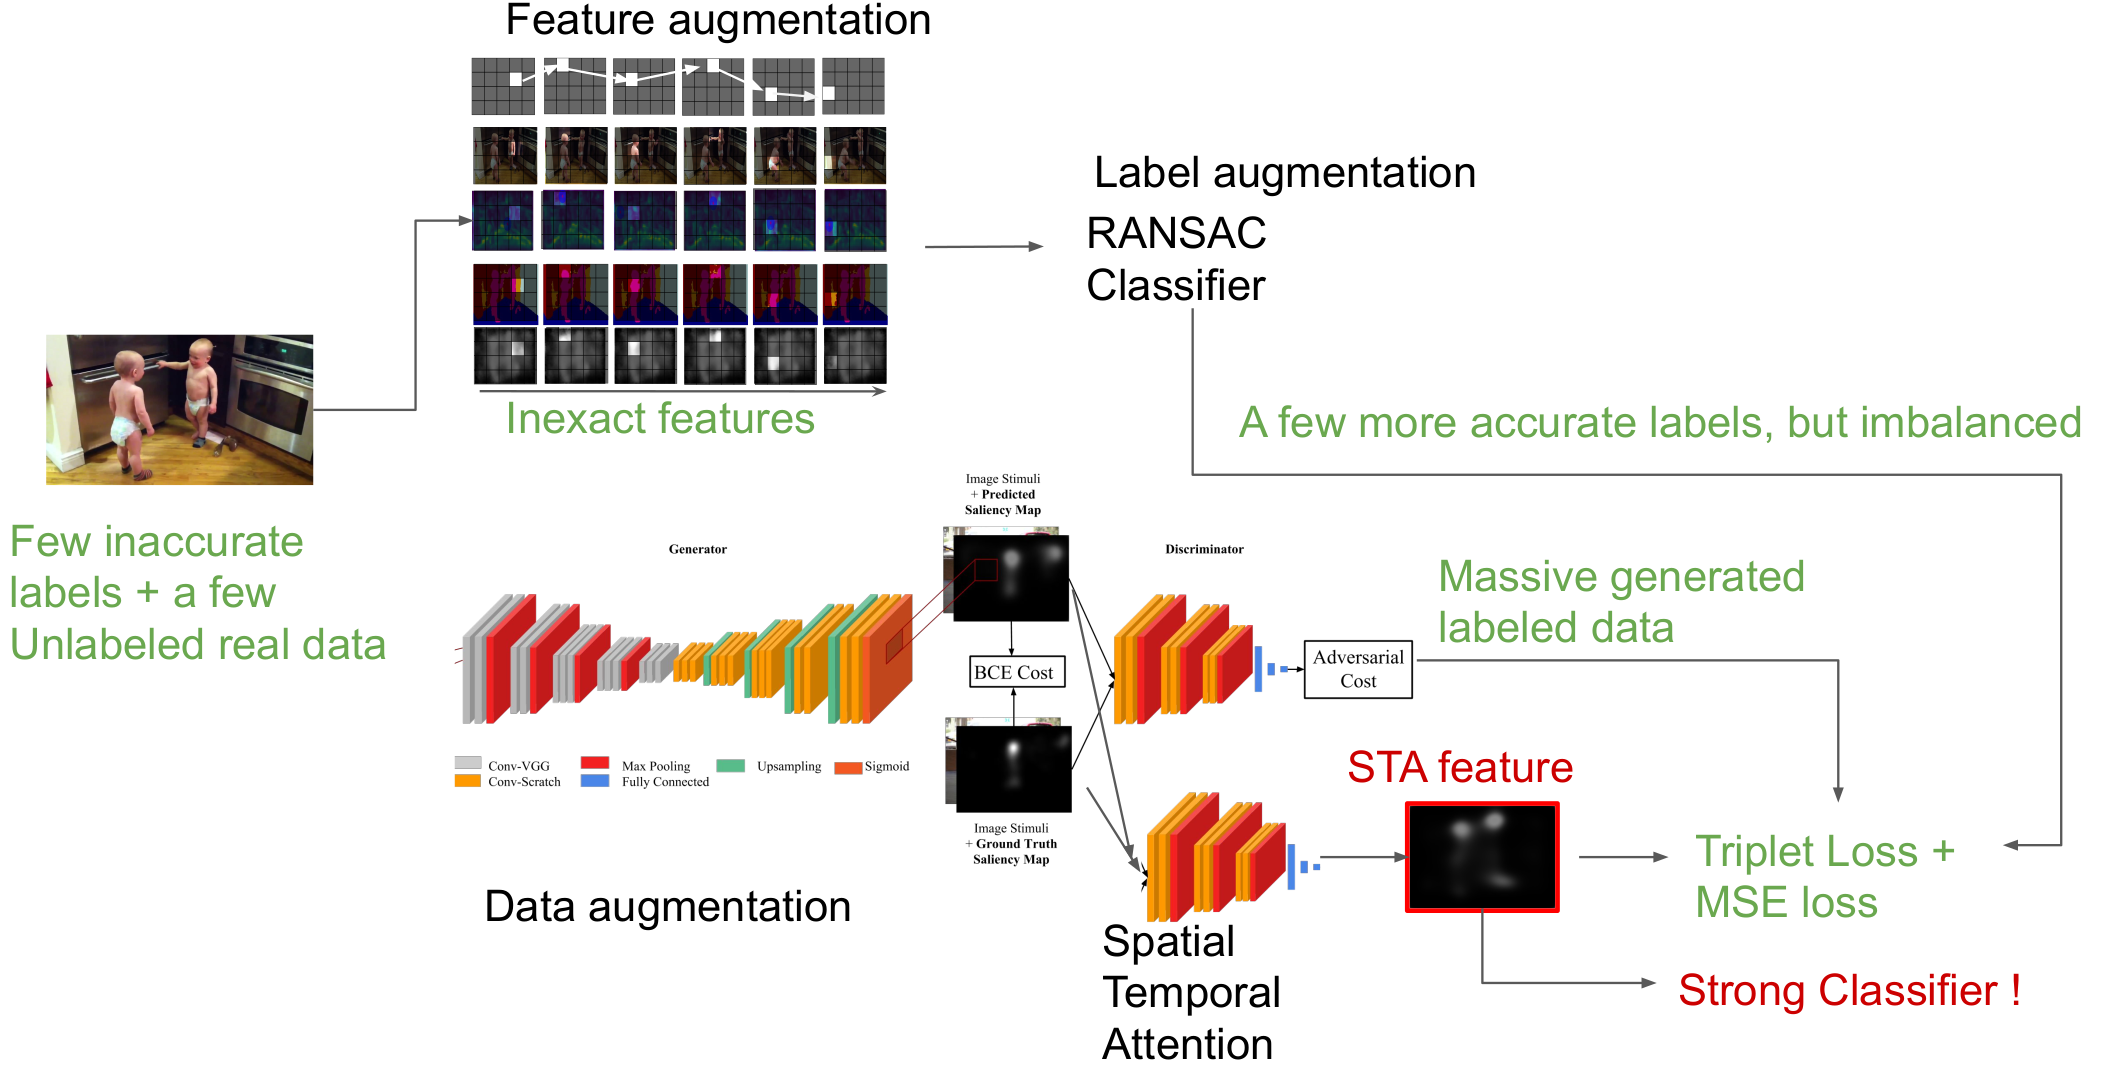
\includegraphics[scale = 0.2]{imgs/future_work.png}
  \caption{ Network Structure of the our future work. The raw clippets are fed in both the RANSAC-SVM module and neural network module. RANSAC module produces pseudo-labels that is used to train neural network(NN) models with a combination of discriminatory loss, reconstruction loss, classification loss, and triplet loss functions. The NN module incorporates a spatial-temporal-attention mechanism that predicts the 4D spatial-temporal saliency map that can be analyzed to help us understand higher level spatial-temporal attention(STA) features that discriminate toxic stress patients and healthy control group. The final STA feature should be a discriminative saliency map that can be used as input as final classification layer. As a result the mAP is greatly improved.}
    \label{fig:baseline}
\end{figure}
\clearpage


\bibliographystyle{plain} % We choose the "plain" reference style
\bibliography{references.bib} % Entries are in the "refs.bib" file
\end{document}
